\chapter{Proposed Methodology}

\section{System Architecture Overview}
The base research under review \cite{1} proposes an industrial-grade multimodal late-fusion architecture specifically designed to overcome the evasion vulnerabilities inherent in unimodal detection frameworks. Rather than attempting to compress diverse, heterogeneous inputs into a unified latent space via early fusion (which frequently induces training instability, high dimensionality, and catastrophic forgetting), the system implements a decoupled late-fusion pipeline.

As illustrated in the schematic pipeline in Figure \ref{fig:arch}, the system ingests a target URL and processes it across four concurrent, specialized analysis branches:
\begin{enumerate}
\item \textbf{Tabular URL Features \& Registration Metadata Branch (CatBoost)}
\item \textbf{Symbolic Character-Level URL Sequence Branch (1D-CNN)}
\item \textbf{DOM Syntactic \& Source Code Logic Branch (Fine-Tuned CodeBERT)}
\item \textbf{Visual Page Rendering \& Brand Impersonation Branch (EfficientNet-B7)}
\end{enumerate}

\begin{figure}[htbp]
\centering
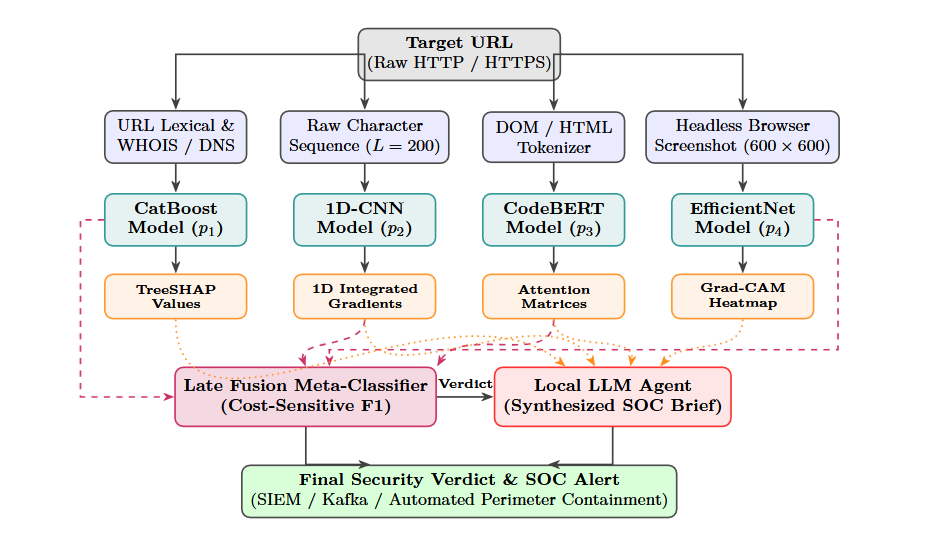
\includegraphics[width=0.95\textwidth]{architecture.png}
\caption{End-to-End Multimodal Late-Fusion Architecture with Explainable AI Subsystems \cite{1}}
\label{fig:arch}
\end{figure}

\section{Modality 1: Tabular URL Features and Metadata via CatBoost}
The first modality processes structured, tabular characteristics extracted from the URL string, DNS servers, and registration authorities.

\subsection{Feature Engineering Pipeline}
A total of 42 engineered features are computed, divided into three categories:
\begin{itemize}
\item \textbf{Lexical URL Attributes:} Total character length, count of numeric digits, ratio of vowel-to-consonant characters, Shannon entropy of the domain string ($H = -\sum_i p_i \log_2 p_i$), count of delimiter symbols (\texttt{.}, \texttt{-}, \texttt{\_}, \texttt{@}, \texttt{=}, \texttt{?}), and presence of sensitive authentication keywords (e.g., \texttt{login}, \texttt{secure}, \texttt{verify}, \texttt{banking}, \texttt{update}).
\item \textbf{Host and Network Attributes:} Number of resolved IPv4/IPv6 addresses, DNS response latency in milliseconds, count of NS (Name Server) and MX (Mail Exchange) records, and Autonomous System Number (ASN) reputation scores.
\item \textbf{Registration and Cryptographic Metadata:} WHOIS domain age (in days since creation), remaining days until domain expiration, registrar country code, and TLS/SSL certificate attributes (issuer authority, validity window, and presence of free automated certificates like Let's Encrypt vs. Extended Validation certificates).
\end{itemize}

\subsection{CatBoost Classification Model}
To model these tabular features, the framework deploys CatBoost (Categorical Boosting) \cite{8}. CatBoost is an open-source gradient boosted decision tree algorithm specifically designed to handle heterogeneous numerical and categorical variables without requiring pre-computed one-hot encodings. It employs Ordered Boosting to eliminate target leakage and utilizes symmetric (oblivious) decision trees as base predictors, ensuring lightning-fast CPU inference times ($< 15\text{ ms}$) and high resilience against overfitting. The output of this branch is a scalar probability $p_{\text{CatBoost}} \in [0, 1]$.

\section{Modality 2: Character-Level Symbolic URL via 1D-CNN}
While feature engineering captures known heuristic properties, it cannot detect novel, obscure string permutations generated by automated phishing kits. The second modality analyzes raw, unprocessed URL character strings using a 1D Convolutional Neural Network (1D-CNN) \cite{1,4}.

\subsection{Character Representation}
Each input URL is truncated or padded to a fixed sequence length $L = 200$ characters. Characters are mapped to indices using an alphabet of 96 printable ASCII characters. Each character index is projected into a dense $d$-dimensional embedding space ($d = 64$):
\begin{equation}
E \in \mathbb{R}^{L \times d}
\label{eq:embed}
\end{equation}

\subsection{Convolutional Feature Extraction}
The embedded sequence $E$ is processed through multiple parallel 1D convolutional filter banks with kernel sizes $k \in \{3, 5, 7\}$ to capture localized n-gram character relationships (e.g., detecting deceptive substrings such as \texttt{micros0ft} or \texttt{paypa1}). The convolution operation for a window of size $k$ produces a feature map:
\begin{equation}
c_i^{(k)} = \text{ReLU}\left(W^{(k)} * E_{i:i+k-1} + b^{(k)}\right)
\label{eq:conv}
\end{equation}

A 1D Global Max-Pooling layer follows each convolutional bank, capturing the most dominant pattern across the entire URL sequence regardless of its exact spatial position:
\begin{equation}
\hat{c}^{(k)} = \max_{1 \le i \le L-k+1} c_i^{(k)}
\label{eq:pool}
\end{equation}

The pooled vectors are concatenated, passed through a fully connected dense layer with Dropout ($p = 0.3$), and activated via a sigmoid neuron to output the scalar probability $p_{\text{CNN1D}}$.

\section{Modality 3: HTML Source Code Representation via Fine-Tuned CodeBERT}
Adversaries frequently employ deceptive Document Object Model (DOM) elements, such as injecting fake credential entry forms that dispatch submitted passwords to external, unauthenticated endpoints. To parse this structural programming logic, the third modality fine-tunes CodeBERT \cite{6}.

\subsection{Transformer Architecture and Pre-training}
CodeBERT is a multi-layer bidirectional Transformer based on the RoBERTa architecture, pre-trained on dual modalities of natural language and source code in multiple programming languages. Unlike generic linguistic models such as BERT, CodeBERT inherently captures syntactic dependencies, variable scoping, and programming idioms.

\subsection{DOM Preprocessing and Tokenization}
The raw HTML document is extracted during crawling. Whitespace redundancies and inline binary assets (e.g., base64 images) are pruned. The cleaned source code is tokenized using Byte-Pair Encoding (BPE) with a sequence length of 512 tokens. A special classification token \texttt{[CLS]} is prepended to the sequence.

During fine-tuning, the final hidden state corresponding to the \texttt{[CLS]} token, denoted $h_{\text{[CLS]}} \in \mathbb{R}^{768}$, is passed through a classification head:
\begin{equation}
p_{\text{CodeBERT}} = \sigma\left(W_{\text{code}} h_{\text{[CLS]}} + b_{\text{code}}\right)
\label{eq:codebert}
\end{equation}
This allows the model to identify concealed deceptive attributes, such as \texttt{<form} \texttt{action=} \allowbreak \texttt{"http://malicious-collector.ru">} nested within seemingly legitimate CSS wrapper templates.

\section{Modality 4: Screenshot-Based Visual Analysis via EfficientNet-B7}
The visual presentation of a website represents the primary vector of deception perceived by the human victim. Attackers frequently replicate high-profile brand landing pages (e.g., Microsoft 365, PayPal, Bank of America) with pixel-level fidelity while hosting them on randomly generated domain names.

\subsection{Image Capture and Normalization}
The target website is rendered inside an automated headless Chromium browser sandbox with a standardized viewport resolution of $1920 \times 1080$. A full-viewport screenshot is captured, normalized across RGB channels, and resized to $600 \times 600 \times 3$.

\subsection{EfficientNet-B7 Backbone}
To analyze visual brand impersonation, the framework utilizes EfficientNet-B7 \cite{7}. EfficientNet utilizes a systematic compound scaling method that balances network depth, width, and image resolution using a compound coefficient $\phi$:
\begin{equation}
\text{depth: } d = \alpha^\phi, \quad \text{width: } w = \beta^\phi, \quad \text{resolution: } r = \gamma^\phi
\label{eq:effnet}
\end{equation}
subject to $\alpha \cdot \beta^2 \cdot \gamma^2 \approx 2$ and $\alpha \ge 1, \beta \ge 1, \gamma \ge 1$.

EfficientNet-B7 deploys mobile inverted bottleneck convolutions (MBConv) enhanced with squeeze-and-excitation (SE) optimization. This architecture extracts high-level semantic features corresponding to organizational logos, security badges, input form positions, and brand color distributions, outputting a visual phishing probability $p_{\text{EfficientNet}}$.

\section{Late-Fusion Trainable Meta-Classifier}
The four specialized branches yield an intermediate prediction vector:
\begin{equation}
\mathbf{p} = \begin{bmatrix} p_{\text{CatBoost}} \\ p_{\text{CNN1D}} \\ p_{\text{CodeBERT}} \\ p_{\text{EfficientNet}} \end{bmatrix} \in [0, 1]^4
\label{eq:pvec}
\end{equation}

Rather than utilizing static heuristic voting, the base study implements a trainable meta-classifier (logistic regression with $L_2$ regularization and gradient boosted decision stumps). The meta-classifier learns the optimal confidence weighting for each modality.

\subsection{Cost-Sensitive Optimization}
Because benign websites vastly outnumber phishing websites in real-world network traffic, training under standard binary cross-entropy induces severe class-imbalance bias. To optimize specifically for the minority phishing class, the meta-classifier is trained under a cost-sensitive weighted loss function:
\begin{equation}
\mathcal{L}_{\text{cost}} = -\frac{1}{N} \sum_{i=1}^N \left[\omega_{\text{phish}} \cdot y_i \log(\hat{y}_i) + (1 - y_i) \log(1 - \hat{y}_i)\right]
\label{eq:cost_loss}
\end{equation}
where $y_i \in \{0, 1\}$ is the ground-truth label, $\hat{y}_i$ is the ensemble prediction, and $\omega_{\text{phish}} > 1$ penalizes false negatives, directly maximizing the operational F1-score.

Furthermore, late fusion provides exceptional operational fault tolerance: if a website is unreachable (rendering screenshot capture impossible), the system handles the missing modality via neutral imputation ($p_{\text{EfficientNet}} = 0.5$), allowing the remaining three branches to render a high-confidence verdict without pipeline failure.

\section{Multimodal Explainable AI (XAI) Suite}
To transform the system from an inscrutable black-box into a transparent decision-support engine, each underlying model is paired with a tailored XAI methodology:
\begin{enumerate}
\item \textbf{TreeSHAP for CatBoost:} Shapley Additive Explanations \cite{9} compute the exact additive marginal contribution $\phi_j$ of each tabular feature:
\begin{equation}
f(x) = \phi_0 + \sum_{j=1}^M \phi_j
\label{eq:shap}
\end{equation}
Features such as ``domain age $< 5$ days'' or ``entropy $> 4.2$'' are assigned quantifiable numerical hazard ratings.

\item \textbf{1D Integrated Gradients for 1D-CNN:} Integrated Gradients \cite{11} computes the path integral of gradients along the straight line from a neutral baseline embedding $x'$ (zero-vector) to the input character sequence $x$:
\begin{equation}
\text{IG}_i(x) = (x_i - x_i') \times \int_0^1 \frac{\partial F(x' + \alpha(x - x'))}{\partial x_i} \, d\alpha
\label{eq:ig}
\end{equation}
This isolates specific character substrings responsible for typosquatting (e.g., highlighting \texttt{paypa1} in an obfuscated domain).

\item \textbf{Attention Matrix Extraction for CodeBERT:} The multi-head self-attention matrices across the final transformer layers are averaged to identify the HTML tokens receiving the highest attentional mass, pinpointing concealed form actions and malicious external script sources.

\item \textbf{Grad-CAM for EfficientNet-B7:} Gradient-weighted Class Activation Mapping \cite{10} calculates gradients of the phishing class score $y^c$ with respect to the feature map activations $A^k$ of the final convolutional layer:
\begin{equation}
\alpha_k^c = \frac{1}{Z} \sum_i \sum_j \frac{\partial y^c}{\partial A_{i,j}^k}
\label{eq:gradcam}
\end{equation}
The resulting heatmap $L_{\text{Grad-CAM}}^c = \text{ReLU}\left(\sum_k \alpha_k^c A^k\right)$ visually illuminates copied brand logos and deceptive credential submission buttons.
\end{enumerate}

\section{Local LLM Agent for Consolidated Incident Reporting}
Raw mathematical attributions (SHAP values, gradient tensors, and heatmap coordinates) are notoriously difficult for human security analysts to parse during active incident triage. To bridge this cognitive gap, the architecture deploys a local Large Language Model (LLM) agent (e.g., quantized Llama-3-8B / Mistral-7B).

The LLM operates under a deterministic system prompt that ingests the JSON payload containing the quantitative XAI attributions and outputs a structured natural language threat intelligence brief. The system is further augmented with Retrieval-Augmented Generation (RAG) connected to an offline database of MITRE ATT\&CK techniques (e.g., T1566: Phishing, T1556: Modify Auth) and historical threat actor profiles. This produces a concise, contextualized incident justification:

\begin{quote}
\textit{``Alert: Confirmed Phishing (Confidence: 98.9\%). The target domain impersonates Microsoft 365. CatBoost flags extreme domain youth (created 2 days ago via automated Let's Encrypt SSL). 1D-CNN identifies character typosquatting in subpath (\texttt{micros0ft-login}). CodeBERT highlights an external credential exfiltration endpoint routed to an untrusted IP address. Grad-CAM confirms exact visual duplication of the official Microsoft corporate login logo.''}
\end{quote}

\section{Microservice Deployment and SIEM Streaming Pipeline}
To ensure industrial scalability, the architecture is implemented as an asynchronous microservice mesh containerized with Docker and orchestrated via Kubernetes. Streaming events from enterprise mail transfer agents (MTAs), web proxies, and endpoint telemetry are ingested via an Apache Kafka distributed message bus. Asynchronous worker pools process URLs concurrently, completing classification within an average end-to-end latency of $120\text{ ms}$. High-severity alerts are published directly to enterprise SIEM dashboards (e.g., Splunk, IBM QRadar), allowing automated firewall perimeter blocking.
